\documentclass[11pt]{article}

\usepackage{amsmath,amssymb,graphicx,geometry,hyperref}

\hypersetup{
  colorlinks=true,
  linkcolor=blue,
  citecolor=blue,
  urlcolor=blue
}

\geometry{margin=2.5cm}

\title{Catani--Seymour Dipole Subtraction for $pp \to t\bar{t}$ at NLO QCD}
\author{Mohamad ElMahdi Houmani}
\date{\today}

\begin{document}

\maketitle

\begin{abstract}
I present a complete implementation of the Catani--Seymour dipole subtraction
formalism for the process $pp \to t\bar{t}$ at next-to-leading order in QCD.
The subtraction terms are constructed explicitly and integrated analytically,
allowing for a fully local cancellation of infrared singularities at the
integrand level.

Particular attention is given to the phase-space factorization, momentum
mappings, and the construction of the Monte Carlo integrand, including
multichannel sampling and adaptive VEGAS integration. The implementation
is validated through local cancellation checks in soft and collinear regions,
as well as through comparisons of total cross sections and differential
distributions.

The results show excellent agreement with reference predictions, confirming
the correctness of both the subtraction procedure and its numerical realization.
The full implementation is available at:
\begin{center}    
\url{https://github.com/mahdihoumanii/topcs}.
\end{center}
\end{abstract}

\section{Structure of the NLO Cross Section}

At next-to-leading order (NLO), the cross section receives contributions
from both real-emission processes and virtual loop corrections.
Schematically, the NLO contribution can be written as
\begin{align}
\sigma^{\text{NLO}} =
\int_{m+1} d\sigma^R +
\int_m d\sigma^V.
\end{align}

The real contribution $d\sigma^R$ corresponds to tree-level processes
with one additional parton in the final state, while the virtual contribution
$d\sigma^V$ contains loop corrections to the Born process.

A key difficulty arises because both terms are separately divergent
in four dimensions. The divergences originate from regions where:
\begin{itemize}
    \item a gluon becomes soft (low energy),
    \item two partons become collinear.
\end{itemize}

Although these singularities cancel in the sum of real and virtual contributions,
this cancellation cannot be performed directly because the two terms are defined
on different phase spaces:
\begin{itemize}
    \item $d\sigma^R$ lives in $(m+1)$-particle phase space,
    \item $d\sigma^V$ lives in $m$-particle phase space.
\end{itemize}

To overcome this, the Catani--Seymour subtraction method introduces
a local counterterm $d\sigma^A$ such that:
\begin{align}
\sigma^{\text{NLO}} =
\int_{m+1} \left(d\sigma^R - d\sigma^A \right)
+
\int_m \left(d\sigma^V + \int_1 d\sigma^A \right).
\end{align}

The subtraction term $d\sigma^A$ is constructed to:
\begin{itemize}
    \item reproduce the singular behavior of $d\sigma^R$ point-by-point,
    \item be analytically integrable over the unresolved phase space.
\end{itemize}

This allows:
\begin{itemize}
    \item the difference $(d\sigma^R - d\sigma^A)$ to be finite and evaluated numerically,
    \item the integrated counterterm $\int_1 d\sigma^A$ to cancel the divergences
    of the virtual contribution.
\end{itemize}

As a result, the entire NLO calculation can be performed in four dimensions,
with all infrared singularities properly cancelled.
\input{sections/01_intro}
\section{Infrared Structure of QCD Amplitudes}

The divergences appearing at NLO originate from universal properties
of QCD amplitudes in specific kinematic limits.
These limits are independent of the details of the process and are
completely determined by the gauge structure of the theory.

\subsection{Soft limit}

When a gluon with momentum $q$ becomes soft ($q \to 0$),
the squared matrix element factorizes as
\begin{align}
|M_{m+1}|^2 \xrightarrow{q \to 0}
\sum_{i,k}
\frac{2 p_i \cdot p_k}{(p_i \cdot q)(p_k \cdot q)}
\langle M_m | \mathbf{T}_i \cdot \mathbf{T}_k | M_m \rangle.
\end{align}

This expression is known as the eikonal factor.
It shows that the emission probability becomes singular when the gluon energy
goes to zero, and that the singularity depends on color correlations
between all pairs of hard partons.

\subsection{Collinear limit}

When two partons $i$ and $j$ become collinear,
their momenta satisfy
\begin{align}
p_i \parallel p_j,
\end{align}
and the matrix element behaves as
\begin{align}
|M_{m+1}|^2 \xrightarrow{ij \text{ collinear}}
\frac{1}{p_i \cdot p_j}
P_{ij}(z)
|M_m|^2.
\end{align}

Here, $P_{ij}(z)$ are the Altarelli--Parisi splitting functions,
which describe the probability of a parton splitting into two collinear partons.

\subsection{Interpretation}

These limits show that:
\begin{itemize}
    \item soft divergences are associated with low-energy gluon emission,
    \item collinear divergences arise from parton splittings,
    \item both types of divergences factorize universally.
\end{itemize}

The role of the subtraction method is to construct counterterms
that locally reproduce these singular behaviors, allowing for a stable
numerical evaluation of the real-emission contribution.
\input{sections/03_infrared}
\section{Dipole Subtraction Terms}

The central idea of the Catani--Seymour method is to construct
local counterterms that reproduce the infrared behavior of the
real-emission matrix element in all singular limits.

These counterterms are written as a sum over dipoles:
\begin{align}
d\sigma^A = \sum_{\text{dipoles}} D_{ij,k}.
\end{align}

Each dipole is associated with:
\begin{itemize}
    \item an emitter pair $(i,j)$,
    \item a spectator parton $k$.
\end{itemize}

The role of the spectator is to ensure momentum conservation
and to absorb recoil in the phase-space mapping.

\subsection{General structure of a dipole}

A dipole term has the general form
\begin{align}
D_{ij,k} =
-\frac{1}{2 p_i \cdot p_j}
\langle M_m(\tilde{p}) |
\mathbf{T}_k \cdot \mathbf{T}_{ij}
\, V_{ij,k}
| M_m(\tilde{p}) \rangle,
\end{align}
where:
\begin{itemize}
    \item $\tilde{p}$ denotes mapped $m$-particle momenta,
    \item $\mathbf{T}_i$ are color charge operators,
    \item $V_{ij,k}$ is the dipole splitting kernel.
\end{itemize}

\subsection{Physical interpretation}

Each dipole term is constructed such that:
\begin{itemize}
    \item in the soft limit, it reproduces the eikonal factor,
    \item in the collinear limit, it reproduces the splitting functions,
    \item away from singular regions, it remains finite.
\end{itemize}

The subtraction term is therefore a local approximation of the real matrix element:
\begin{align}
d\sigma^R \approx d\sigma^A \quad \text{in all singular limits}.
\end{align}

\subsection{Local cancellation}

By construction, the difference
\begin{align}
d\sigma^R - d\sigma^A
\end{align}
is finite everywhere in phase space and can be integrated numerically
without encountering divergences.

This local cancellation is the key advantage of the Catani--Seymour method,
as it allows for stable Monte Carlo integration.
\section{Phase Space Factorization and Mapping}

A central ingredient of the Catani--Seymour subtraction method is the
exact factorization of the $(m+1)$-particle phase space into an
$m$-particle phase space and an unresolved emission measure.

\subsection{Phase-space definition}

The $(m+1)$-particle phase space is defined as
\begin{align}
d\Phi_{m+1}(P; p_1,\dots,p_{m+1}) =
\left( \prod_{i=1}^{m+1} \frac{d^3 p_i}{(2\pi)^3 2E_i} \right)
(2\pi)^4 \delta^{(4)}\!\left(P - \sum_{i=1}^{m+1} p_i \right).
\end{align}

For subtraction to work, this phase space must be rewritten in terms of
a reduced $m$-particle configuration.

\subsection{Factorization}

For each dipole $(ij,k)$, the phase space can be factorized as
\begin{align}
d\Phi_{m+1}(p_1,\dots,p_{m+1}) =
d\Phi_m(\tilde{p}_1,\dots,\tilde{p}_m)
\, [dp_i(\tilde{p}_{ij}, \tilde{p}_k)],
\end{align}
where:
\begin{itemize}
    \item $\tilde{p}$ denotes mapped momenta,
    \item $[dp_i]$ is the dipole phase-space measure associated with the
    unresolved emission.
\end{itemize}

This factorization is exact and includes a non-trivial Jacobian.

\subsection{Momentum mapping}

The mapping $(p_i, p_j, p_k) \to (\tilde{p}_{ij}, \tilde{p}_k)$ is constructed such that:
\begin{align}
\tilde{p}_{ij} + \tilde{p}_k = p_i + p_j + p_k,
\end{align}
and:
\begin{align}
\tilde{p}_{ij}^2 = p_{ij}^2, \quad \tilde{p}_k^2 = p_k^2.
\end{align}

A commonly used mapping (final-final case) is:
\begin{align}
\tilde{p}_{ij}^\mu &= p_i^\mu + p_j^\mu - \frac{y_{ij,k}}{1 - y_{ij,k}} p_k^\mu, \\
\tilde{p}_k^\mu &= \frac{1}{1 - y_{ij,k}} p_k^\mu,
\end{align}
with:
\begin{align}
y_{ij,k} = \frac{p_i \cdot p_j}{p_i \cdot p_j + p_j \cdot p_k + p_k \cdot p_i}.
\end{align}

\subsection{Dipole phase-space measure}

The unresolved phase-space factor can be written as
\begin{align}
[dp_i(\tilde{p}_{ij}, \tilde{p}_k)] =
\frac{(1 - y_{ij,k})^{d-3}}{16\pi^2}
\, (p_{ij,k}^2)^{1-\epsilon}
\, dy_{ij,k} \, dz_i \, d\phi,
\end{align}
where:
\begin{itemize}
    \item $y_{ij,k}$ controls the invariant mass of the splitting,
    \item $z_i$ is the energy fraction,
    \item $\phi$ is the azimuthal angle.
\end{itemize}

\subsection{Role in the implementation}

This factorization allows the real-emission contribution to be rewritten as:
\begin{align}
\int d\Phi_{m+1} \, d\sigma^R =
\int d\Phi_m \int [dp_i] \, d\sigma^R.
\end{align}

The subtraction term uses the same mapping, ensuring that:
\begin{itemize}
    \item both $d\sigma^R$ and $d\sigma^A$ are evaluated consistently,
    \item the difference remains finite,
    \item the integrated dipoles can be computed analytically.
\end{itemize}
\section{Integrated Dipoles and Virtual Cancellation}

The subtraction term $d\sigma^A$ is constructed to reproduce the singular
behavior of the real-emission contribution. In order to combine it with
the virtual corrections, it must be integrated analytically over the
unresolved phase space.

\subsection{Integrated subtraction term}

The integration of the subtraction term over the unresolved emission
leads to
\begin{align}
\int_1 d\sigma^A = d\sigma^B \otimes \mathbf{I}.
\end{align}

Here, $\mathbf{I}$ is an operator acting on the Born matrix element,
and it contains explicit poles in dimensional regularization:
\begin{align}
\mathbf{I} \sim \frac{1}{\epsilon^2} + \frac{1}{\epsilon}.
\end{align}

These poles match exactly the infrared divergences of the virtual
contribution $d\sigma^V$.

\subsection{Cancellation of divergences}

The virtual contribution has the structure
\begin{align}
d\sigma^V \sim \frac{1}{\epsilon^2} + \frac{1}{\epsilon} + \text{finite}.
\end{align}

When combined with the integrated subtraction term, the poles cancel:
\begin{align}
d\sigma^V + \int_1 d\sigma^A = \text{finite}.
\end{align}

This cancellation ensures that the virtual contribution can be evaluated
in four dimensions.

\subsection{Initial-state collinear contributions}

For hadronic processes, additional collinear singularities arise from
initial-state radiation. These are absorbed into the parton distribution
functions (PDFs) through mass factorization.

This introduces additional terms, commonly denoted as $\mathbf{P}$ and
$\mathbf{K}$ operators:
\begin{align}
\sigma^{\text{NLO}} \supset \int dx \, \left( \mathbf{P} + \mathbf{K} \right).
\end{align}

\begin{itemize}
    \item The $\mathbf{P}$ term is related to Altarelli--Parisi splitting
    functions and governs the scale dependence of PDFs.
    \item The $\mathbf{K}$ term contains finite remainders from the
    factorization procedure.
\end{itemize}

\subsection{Interpretation}

The integrated dipoles complete the subtraction procedure:
\begin{itemize}
    \item they cancel the infrared poles of the virtual corrections,
    \item they account for initial-state collinear singularities,
    \item they ensure that the full NLO result is finite.
\end{itemize}
\section{Implementation Strategy}

The subtraction formalism is implemented at the level of the Monte Carlo
integrand, where each phase-space point contributes a finite weight.
Particular care is taken to follow closely the structure of modern
integrators such as the Munich framework used in MATRIX.

\subsection{Monte Carlo weight}

At each phase-space point, the weight is given by
\begin{align}
w =
\frac{1}{2\hat{s}} \,
f_a(x_1,\mu_F) \, f_b(x_2,\mu_F)
\, d\Phi \,
\alpha_s^n(\mu_R)
\, |M|^2,
\end{align}
where $\hat{s} = x_1 x_2 s$ and $d\Phi$ includes all Jacobians from the
phase-space mappings.

\subsection{Local subtraction at the integrand level}

The real-emission contribution is evaluated as
\begin{align}
\mathcal{R}_{\text{finite}} =
|M_{m+1}|^2 - \sum_{\text{dipoles}} D_{ij,k},
\end{align}
which is finite at every phase-space point.

The virtual contribution is combined with the integrated dipoles:
\begin{align}
\mathcal{V}_{\text{finite}} =
|M_m^{\text{1-loop}}|^2 + \langle M_m | \mathbf{I} | M_m \rangle.
\end{align}

\subsection{Multichannel phase-space sampling}

Following the strategy used in Munich, the phase space is sampled using
a multichannel approach. The idea is to construct a probability density
as a weighted sum over different phase-space channels:
\begin{align}
g_{\text{MC}}(x) = \sum_c \alpha_c \, g_c(x),
\end{align}
where:
\begin{itemize}
    \item $g_c(x)$ are individual channel densities adapted to specific
    kinematic structures (e.g. soft or collinear regions),
    \item $\alpha_c$ are channel weights satisfying $\sum_c \alpha_c = 1$.
\end{itemize}

Each channel is designed to capture a particular singular behavior of
the matrix element, improving the efficiency of the integration.

\subsection{Adaptive integration (VEGAS)}

On top of the multichannel structure, an adaptive VEGAS algorithm is used
to refine the sampling of the integration variables.

The VEGAS procedure builds an importance-sampling grid for each integration
dimension, iteratively updating the sampling density according to
\begin{align}
g(x) \propto |w(x)|.
\end{align}

This allows the integrator to concentrate sampling in regions where the
integrand is large, such as near infrared-sensitive configurations.

\subsection{Combination of multichannel and VEGAS}

The final sampling density is given by the combination of both strategies:
\begin{itemize}
    \item the multichannel decomposition captures the global structure
    of the phase space,
    \item the VEGAS adaptation refines the sampling locally.
\end{itemize}

This mirrors the approach used in Munich, where both techniques are used
together to achieve stable and efficient integration of NLO contributions.

\subsection{Hadronic convolution}

The hadronic cross section is obtained as
\begin{align}
\sigma =
\sum_{a,b} \int dx_1 dx_2 \,
f_a(x_1,\mu_F) f_b(x_2,\mu_F)
\left[
\int d\Phi_{m+1} \, \mathcal{R}_{\text{finite}}
+
\int d\Phi_m \, \mathcal{V}_{\text{finite}}
\right].
\end{align}

\subsection{Numerical stability}

The combination of local subtraction, multichannel sampling,
and adaptive VEGAS integration ensures that:
\begin{itemize}
    \item the integrand remains finite across the entire phase space,
    \item singular regions are efficiently sampled,
    \item the Monte Carlo integration converges reliably.
\end{itemize}
\section{Validation and Consistency Checks}

To ensure the correctness of the implementation, several validation
tests were performed at the level of individual phase-space points
and integrated quantities.

\subsection{Local cancellation of singularities}

A central check of the subtraction procedure is the local cancellation
between the real-emission matrix element and the dipole subtraction terms.

At fixed phase-space points approaching soft or collinear regions,
we evaluate:
\begin{align}
\mathcal{R}_{\text{finite}} =
|M_{m+1}|^2 - \sum_{\text{dipoles}} D_{ij,k}.
\end{align}

Numerically, it is observed that:
\begin{itemize}
    \item both $|M_{m+1}|^2$ and the dipole sum become large in singular regions,
    \item their difference remains finite,
    \item the cancellation occurs point-by-point.
\end{itemize}

This confirms that the dipole terms correctly reproduce the infrared
structure of the real matrix element.

\subsection{Behavior near singular limits}

To further verify the implementation, phase-space points were generated
close to soft and collinear configurations.

In these regions:
\begin{itemize}
    \item the real matrix element exhibits the expected singular growth,
    \item the dipole terms follow the same scaling behavior,
    \item the subtracted quantity remains stable.
\end{itemize}

This demonstrates that the subtraction is correctly capturing the
leading singular behavior.

\subsection{Cancellation of virtual poles}

The combination
\begin{align}
\mathcal{V}_{\text{finite}} =
|M_m^{\text{1-loop}}|^2 + \langle M_m | \mathbf{I} | M_m \rangle
\end{align}
was verified to be finite.

In particular:
\begin{itemize}
    \item the $1/\epsilon^2$ and $1/\epsilon$ poles cancel,
    \item the resulting expression is well-defined in four dimensions.
\end{itemize}

This confirms the consistency between the integrated dipoles and
the virtual corrections.

\subsection{Numerical stability}

The full integrand was tested across a wide range of phase-space points.

It is observed that:
\begin{itemize}
    \item the real-emission contribution remains finite after subtraction,
    \item no numerical instabilities appear in soft or collinear regions,
    \item the Monte Carlo integration converges smoothly.
\end{itemize}

\subsection{Summary of validation}

These checks demonstrate that:
\begin{itemize}
    \item the dipole subtraction terms are correctly implemented,
    \item the phase-space mappings are consistent,
    \item the cancellation of infrared singularities is achieved locally
    and globally.
\end{itemize}
\section{Results}

In this section, we present the numerical results obtained from the
implementation, including total cross sections and differential
distributions.

\subsection{Total cross sections}

The NLO cross section for $pp \to t\bar{t}$ was computed at two
center-of-mass energies, using the NNPDF3.1 NLO PDF set with
$\alpha_s = 0.118$ and renormalization and factorization scales
set to $\mu_R = \mu_F = m_t = 173~\text{GeV}$.

At $\sqrt{s} = 8~\text{TeV}$, we obtain:
\begin{align}
\sigma_{\text{NLO}} = 220.666 \pm 0.552~\text{pb},
\end{align}
to be compared with the Top++ prediction:
\begin{align}
\sigma_{\text{Top++}} = 220.689~\text{pb}.
\end{align}

At $\sqrt{s} = 13~\text{TeV}$, we obtain:
\begin{align}
\sigma_{\text{NLO}} = 731.972 \pm 0.6211~\text{pb},
\end{align}
to be compared with:
\begin{align}
\sigma_{\text{Top++}} = 732.912~\text{pb}.
\end{align}

The agreement at the level of $\mathcal{O}(10^{-2})$ pb demonstrates
the correctness of the implementation and the normalization.

\subsection{Differential distributions}

We also computed several differential distributions at LO and NLO
and compared them with reference results.

\subsubsection{Invariant mass distribution}

The invariant mass distribution of the top-quark pair is shown in
Fig.~\ref{fig:mtt_lo} and Fig.~\ref{fig:mtt_nlo}.

\begin{figure}[h!]
\centering
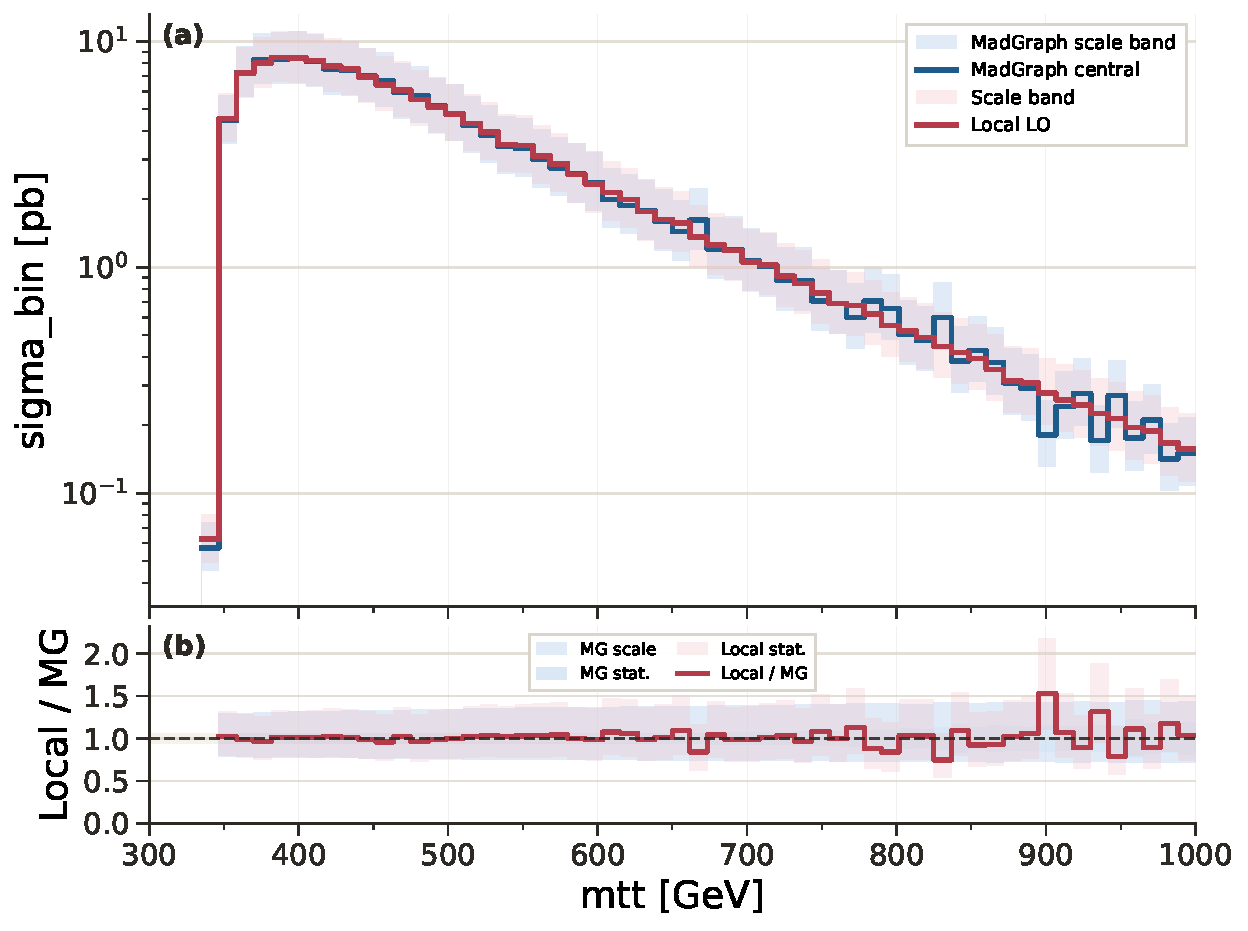
\includegraphics[width=0.4\textwidth]{figures/mtt_lo_vs_madgraph.pdf}
\caption{Invariant mass distribution at LO compared to MadGraph.}
\label{fig:mtt_lo}
\end{figure}

\begin{figure}[h!]
\centering
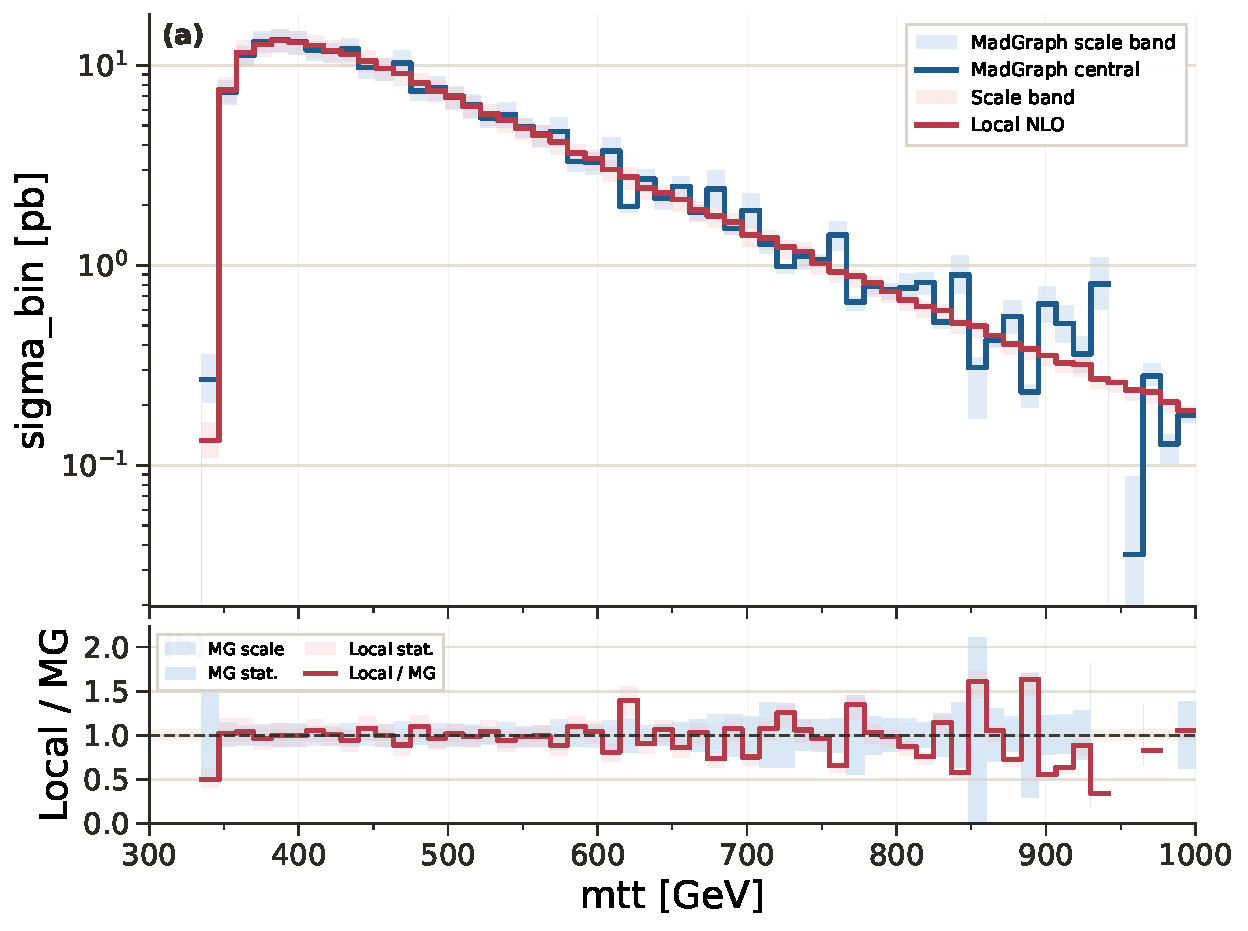
\includegraphics[width=0.4\textwidth]{figures/mtt_nlo_vs_madgraph.pdf}
\caption{Invariant mass distribution at NLO compared to reference results.}
\label{fig:mtt_nlo}
\end{figure}

\subsubsection{Top transverse momentum}

The transverse momentum distribution of the top quark is shown in
Fig.~\ref{fig:pt_lo} and Fig.~\ref{fig:pt_nlo}.

\begin{figure}[h!]
\centering
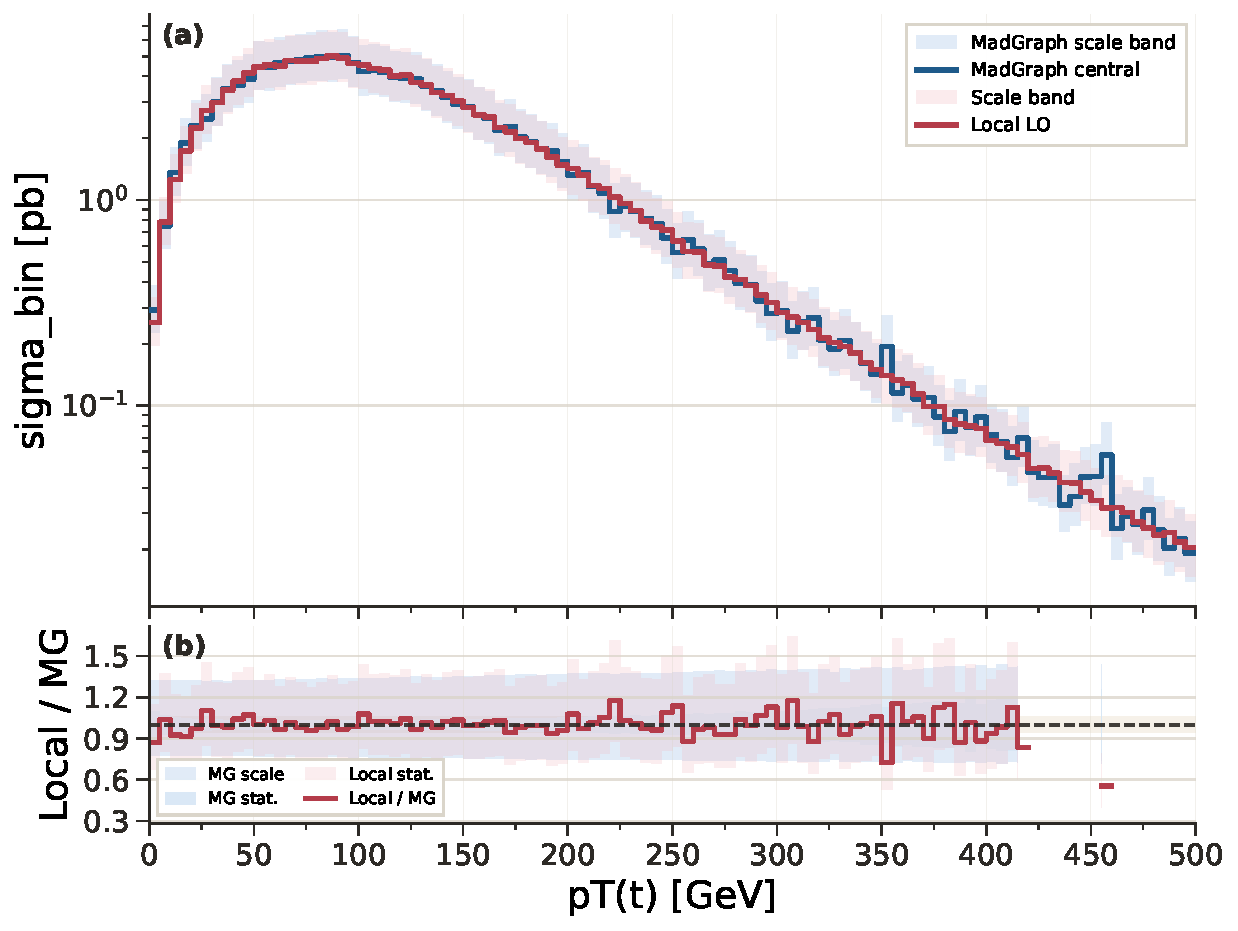
\includegraphics[width=0.4\textwidth]{figures/top_pt_lo_vs_madgraph.pdf}
\caption{Top $p_T$ distribution at LO compared to MadGraph.}
\label{fig:pt_lo}
\end{figure}

\begin{figure}[h!]
\centering
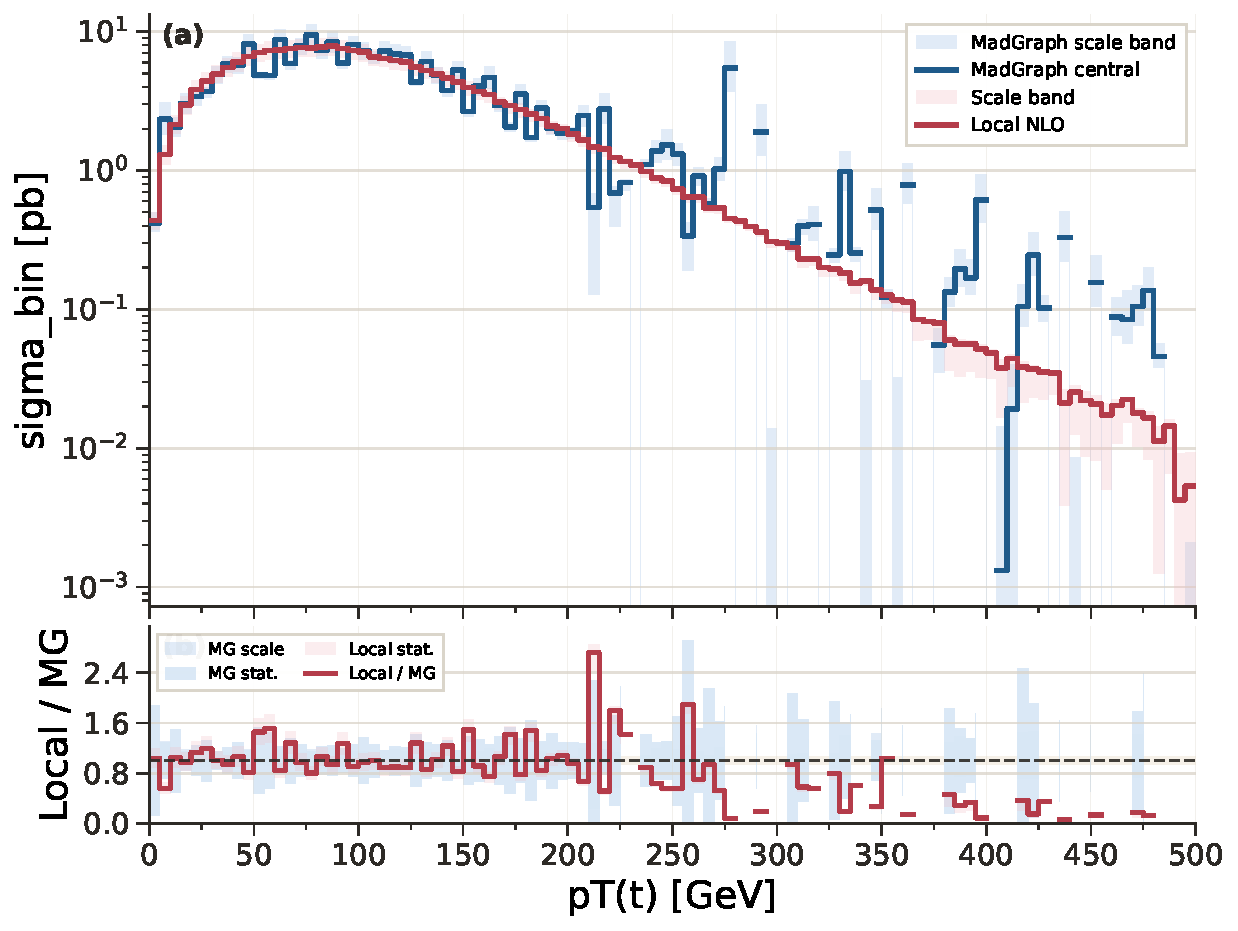
\includegraphics[width=0.4\textwidth]{figures/top_pt_nlo_vs_madgraph.pdf}
\caption{Top $p_T$ distribution at NLO.}
\label{fig:pt_nlo}
\end{figure}

\subsubsection{Rapidity distribution}

The rapidity distribution of the $t\bar{t}$ system is shown in
Fig.~\ref{fig:ytt_lo} and Fig.~\ref{fig:ytt_nlo}.

\begin{figure}[h!]
\centering
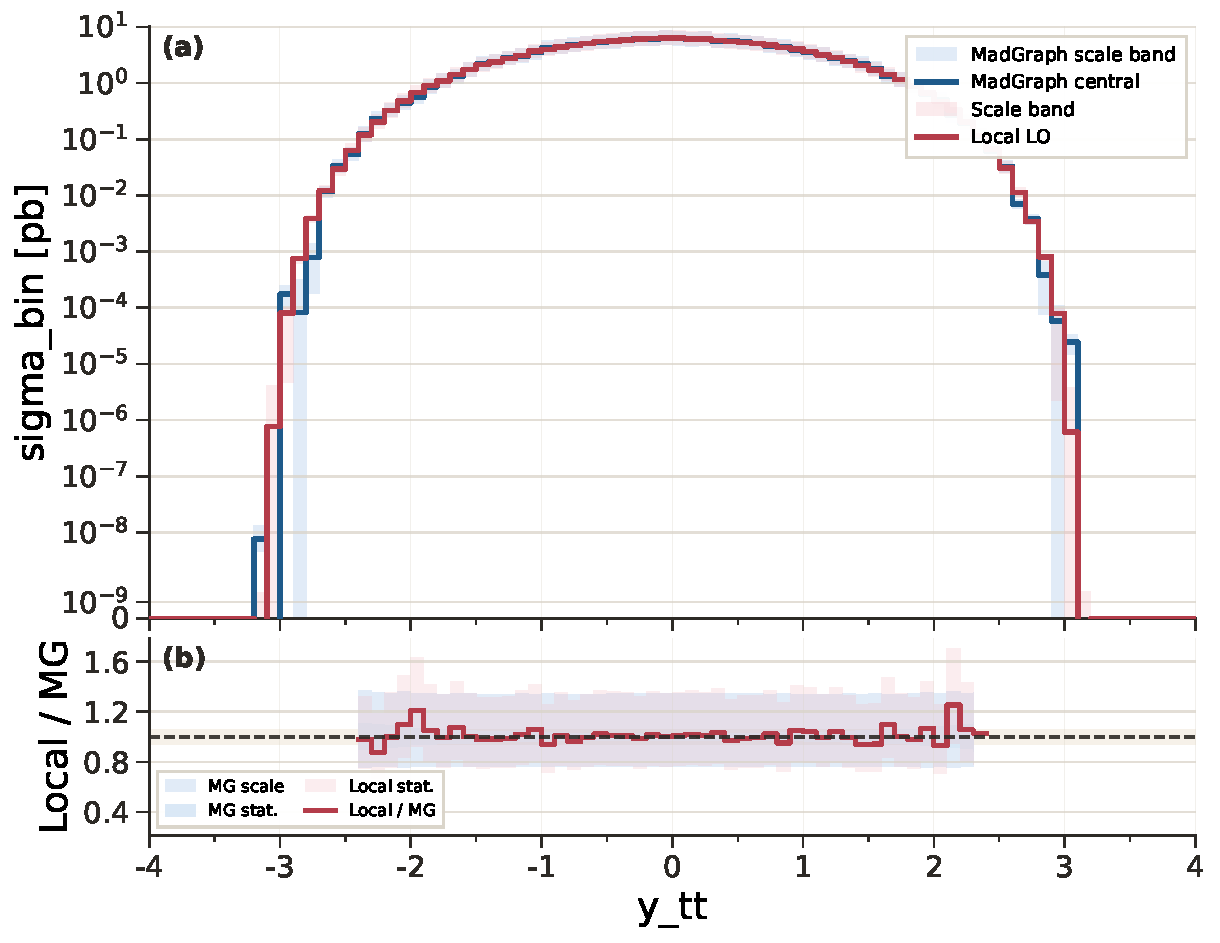
\includegraphics[width=0.4\textwidth]{figures/ytt_lo_vs_madgraph.pdf}
\caption{Rapidity distribution at LO.}
\label{fig:ytt_lo}
\end{figure}

\begin{figure}[h!]
\centering
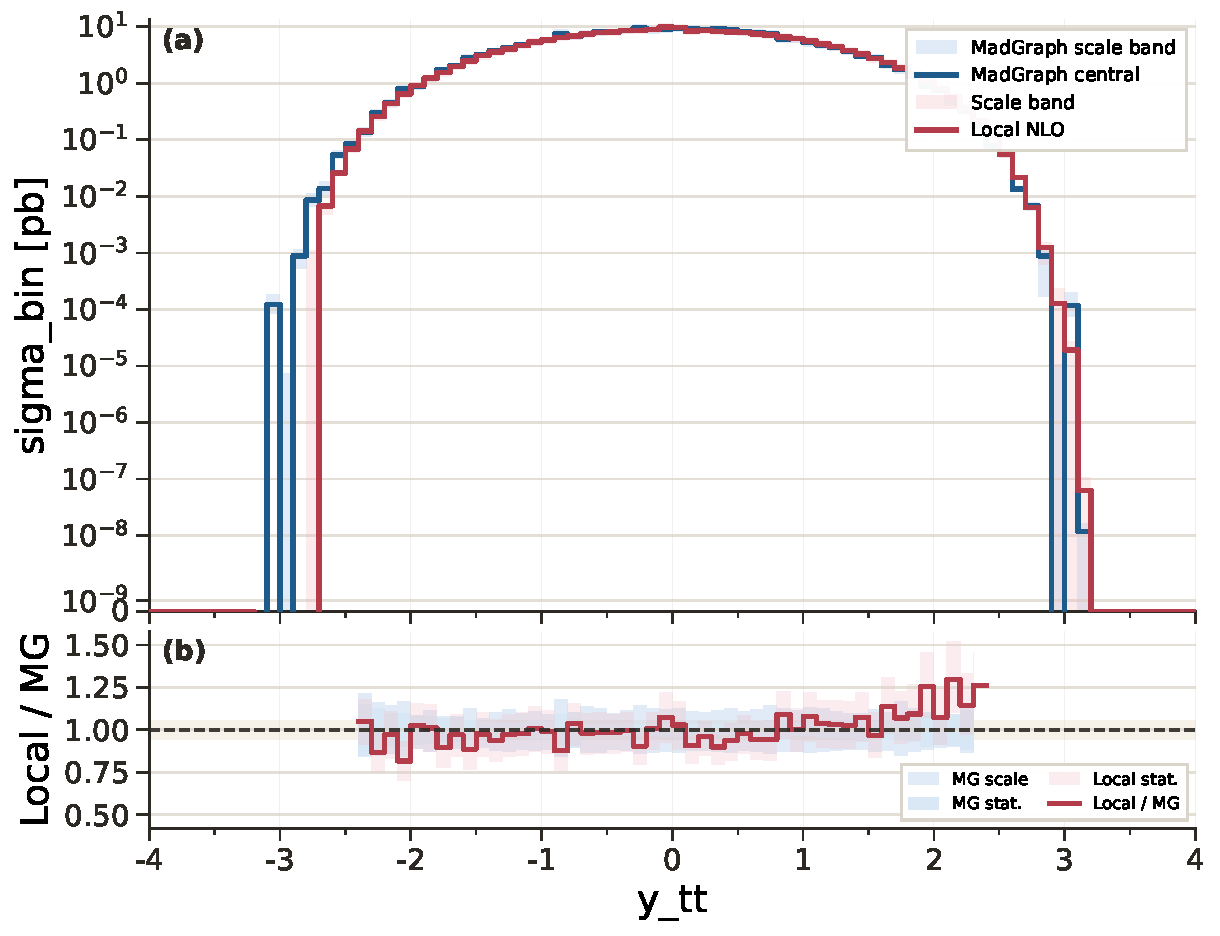
\includegraphics[width=0.4\textwidth]{figures/ytt_nlo_vs_madgraph.pdf}
\caption{Rapidity distribution at NLO.}
\label{fig:ytt_nlo}
\end{figure}

\subsection{Discussion}

The total cross sections show excellent agreement with Top++,
indicating that both the normalization and the subtraction procedure
are correctly implemented.

At the differential level:
\begin{itemize}
    \item LO distributions agree with MadGraph, validating the phase-space
    generation and matrix elements,
    \item NLO corrections modify both normalization and shape,
    \item the distributions remain smooth, confirming numerical stability.
\end{itemize}

Overall, these results demonstrate that the implementation correctly
reproduces both inclusive and differential observables at NLO.

\end{document}